\section{Result}
\begin{figure*}[ht]
\center
  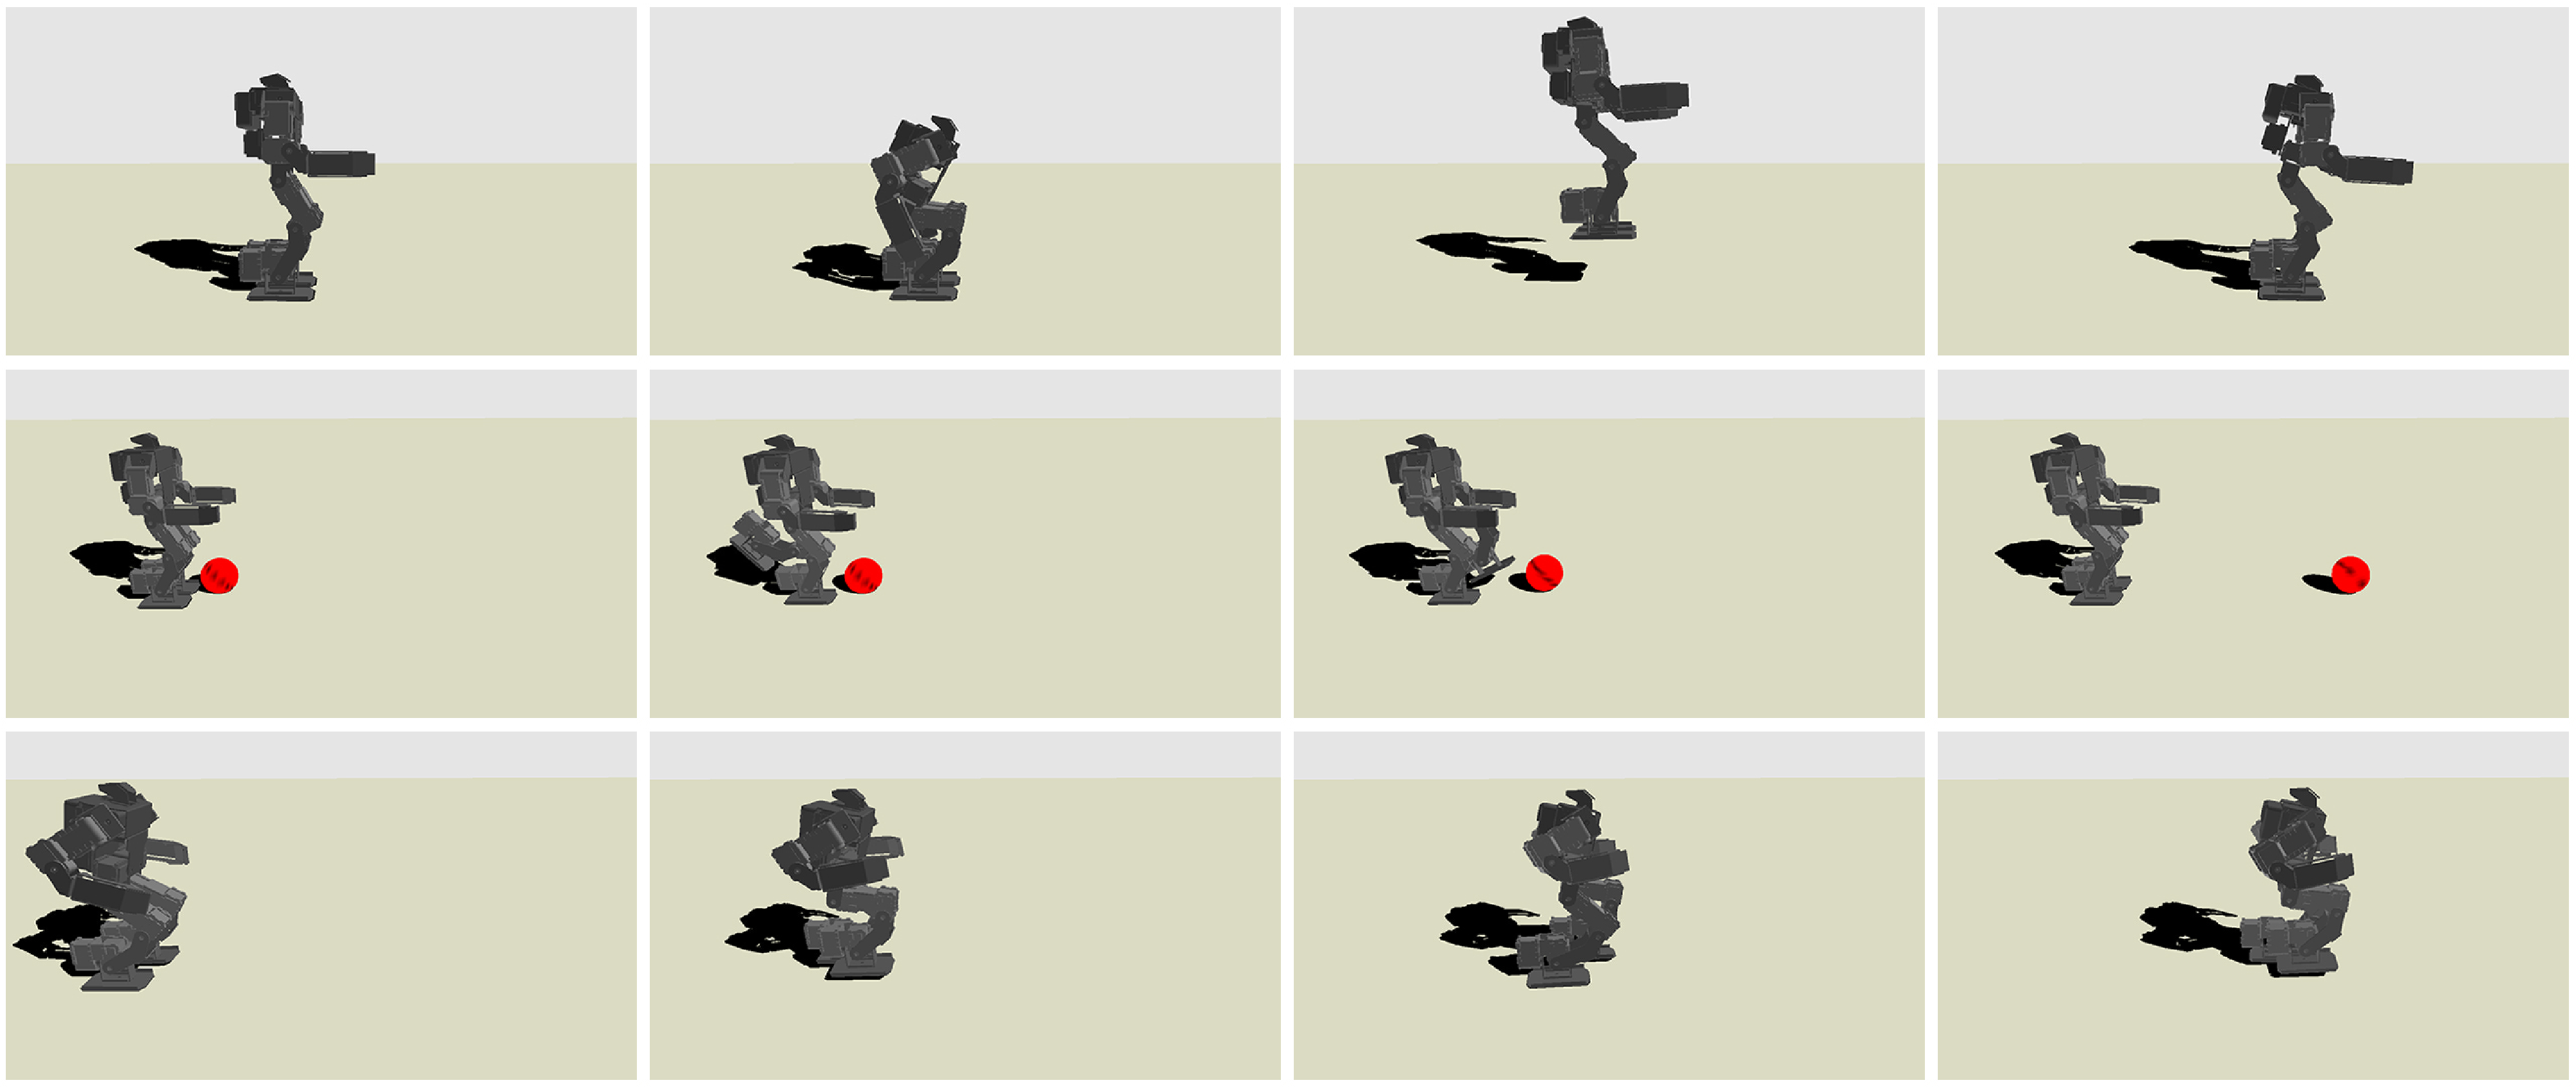
\includegraphics[width=0.95\textwidth]{images/motions}
  \caption{
Top: Vertical jump with parameterized target height, $3cm$ to
      $8cm$ ($8cm$ is shown).
      Middle: Kick with parameterized target distance, $0.3m$ to $0.6m$
      ($0.6m$ is shown).
      Bottom: Walk with parameterized target speed, $6.7cm/s$ to $13.3cm/s$
      ($13.3cm/s$ is shown).
      %% Middle: kicking with various target distances
      %% Bottom: walking with various target speeds}
    %% \sehoon{1) Robots should be zoomed. 2) Robot colors should be brighter (red
    %%   and orange?)} \karen{Use solid color for the floor instead of
    %%   checkerboard. Zoom in to the robot. Use grayish color for the
    %%   robot. Remove the coordinate frame lines.}
    %% \sehoon{Got it.}
  }
  \label{fig:optskills_motions}
\end{figure*}

We compared our algorithm and the baseline
algorithm, CMA-ES, on three dynamic motor control problems and four
parameterized CEC'15 problems. The baseline algorithm uses CMA-ES to
search for the mapping parameter $\boldsymbol{\phi}\in\mathcal{F}$ that minimizes the
objective function $\hat{f}(\boldsymbol{\phi})$ (\eqnref{optskills_disccost}),
while our algorithm follows the procedure described in Section
\ref{sec:optskills_our_algorithm}.

For all problems, we measured the
number of sample evaluations and/or the quality of the final
solution. Evaluating a sample in a motor control problem involves
simulating a sequence of motion, which is typically the bottleneck of
using a sampling-based optimizer to solve a control problem. 
%% \karen{Is this enough of justification on our metric?}
%% \sehoon{For me, yes.}
Because of the stochastic nature of our algorithm, for each problem we ran
nine optimization trials with different initial seeds and reported the
average results of seven trials, excluding the best and the worst
trials. Our algorithm generates $\lambda=16$ samples at each
iteration and maintains $\mu=48$ elite samples, while CMA-ES
generates $\lambda_{cma}=16$ samples each iteration and selects
$\mu_{cma}=8$ elite samples.

  %% For each trial of optimization, we have two terminal conditions:
  %% 1) The objective value of the solution segment drops below athreshold, 
  %% or 2) The number of simulation evaluations exceeds the maximum number.}

% \updated{Please note that we measure a number of \emph{simulation samples}
%   ($\mathcal{S}$ in \eqnref{optskills_paramcost}) instead of a number of function
%   evaluation itself.
%   This is because an evaluation of simulation with a given control parameter is
%   a bottle neck of a sampling-based control optimization.
%   Once a simulation $\mathcal{S}$ is acquired, we can easily re-evaluate it
%   with different task parameters.  
%   In mathematical problems, we simply check the number of samples $\vc{x}$ in
%   $\mathcal{X}$ space.}

%%%%%%%%%%%%%%%%%%%%%%%%%%%%%%%%%%%%%%%%%%%%%%%%%%%%%%%%%%%%%%%%%%%%%%%%%%%%%%%%

\subsection{Parameterized Motor Skills}

% \begin{table}[b]
% \center
% {
% %% \small
% \caption{ Cost terms $h(\mathcal{S})$}
% \begin{tabular}{| c | c | }
% \hline
% Cost Term & Description \\ \hline
% $\vc{C}_f(\mathcal{S})$ & The final position of COM: $\vc{C}(\vc{s}_T)$ \\ \hline
% %% $\vc{\dot{C}}_f(\mathcal{S})$ & The final velocity of COM: $\vc{\dot{C}}(\vc{s}_T)$\\ \hline
% $\vc{Y}_{max}(\mathcal{S})$ & The maximum height of COM: $\max_{\vc{s}_i\in\mathcal{S}}{\vc{C}_y(\vc{s}_i)}$\\ \hline
% $\vc{B}_f(\mathcal{S})$ & The final position of the ball: $\vc{B}(\vc{s}_T)$\\ \hline
% %% $\vc{P}$ & The position of the support polygon \\ \hline
% $\vc{Z}(\mathcal{S})$ & The balance: 
% $\sum_{\vc{s}_i\in\mathcal{S}}\|\vc{C}(\vc{s}_i)-\vc{P}(\vc{s}_i)\|^2$ \\ \hline
% \end{tabular}
% \label{tab:optskills_cost}
% }
% \end{table}

The primary goal of this work is to learn controllers for
parameterized dynamic motor skills.  We experimented three dynamic
tasks, vertical jump, kick a ball, and walk (\figref{optskills_motions}), on a small
humanoid, BioloidGP \cite{BioloidGP:2014:URL} ($34.6cm$ and $1.6kg$).
All motions were simulated using an open source physics engine, DART
\cite{DART:2014:URL,Liu:2012:STM}, with $0.0005s$ as the simulation
time step. We set the joint angle limits at $\pm150^{\circ}$ and the
torque limits at $0.6Nm$. Contact and collision were handled using
implicit time-stepping, velocity-based LCP (linear-complementarity
problem) to guarantee non-penetration, directional friction, and
approximated Coulomb friction cone conditions.

The parameterized walking skill was also demonstrated on the
hardware. Please see the supplementary video for simulated motion
sequences and recorded video footages.

We used two simple control mechanisms to define the policy parameter
space and let our algorithm find the optimal policy. The first control
mechanism is to use PD servos to track target poses. The second one
is to control the desired force a body link exerts to the world using
Jacobian transpose \cite{Sunada:1994:ACJ}. The definitions of cost function
vary by tasks and will be described in the following subsections.

\begin{figure}
\center
  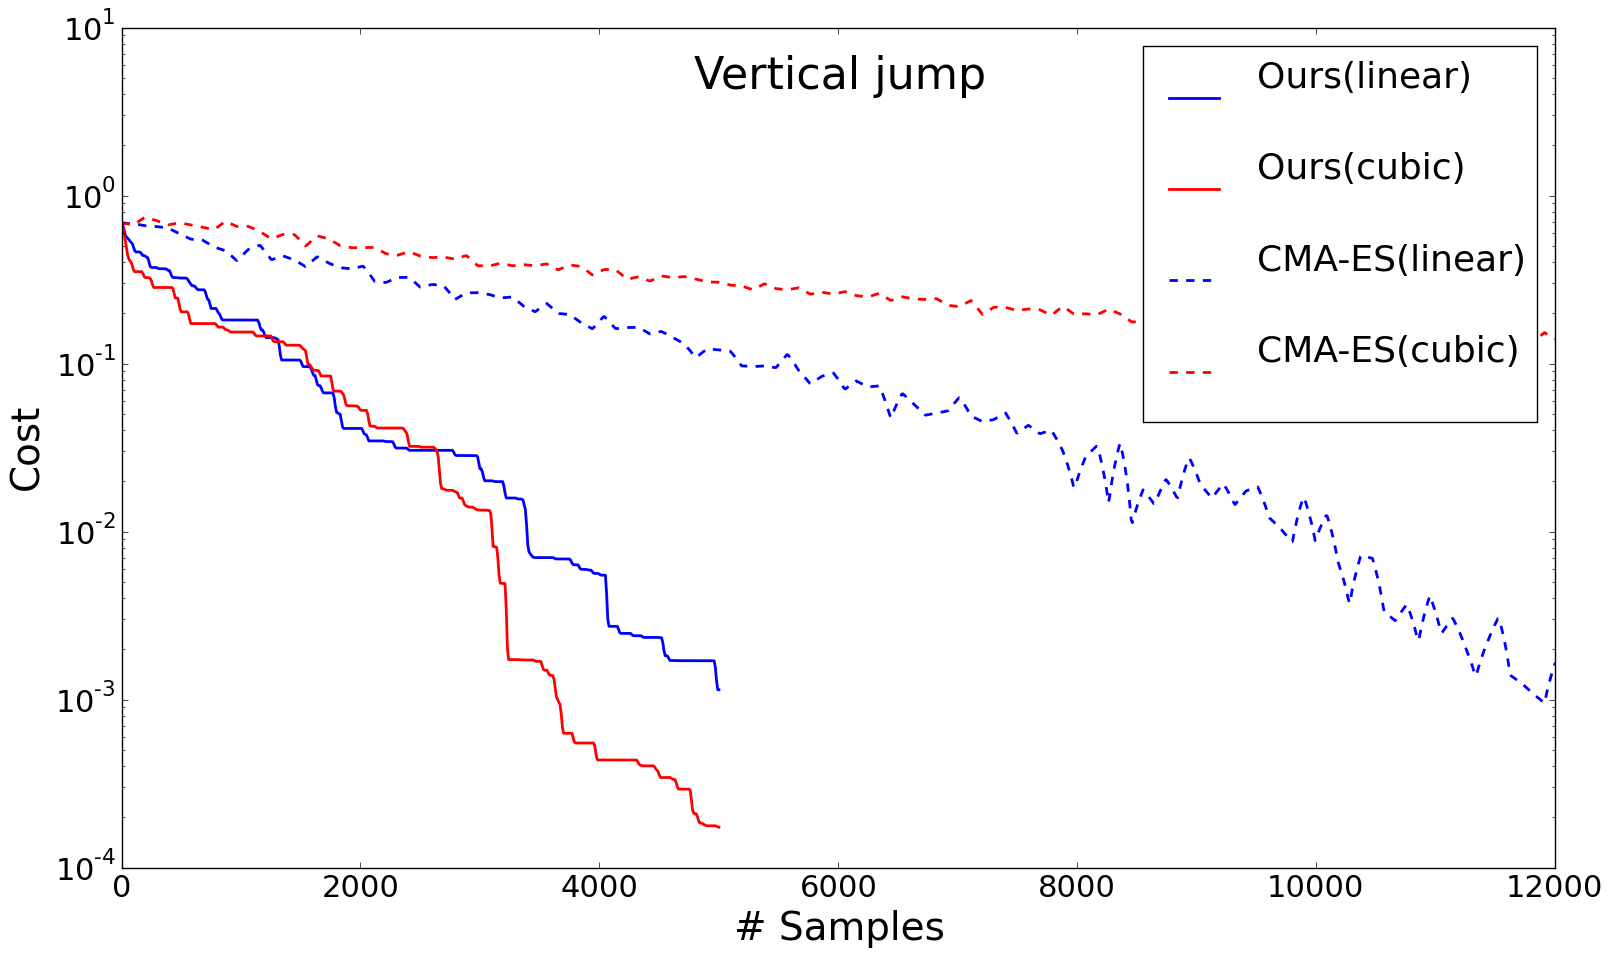
\includegraphics[width=4.5in]{images/iter_values_00}
  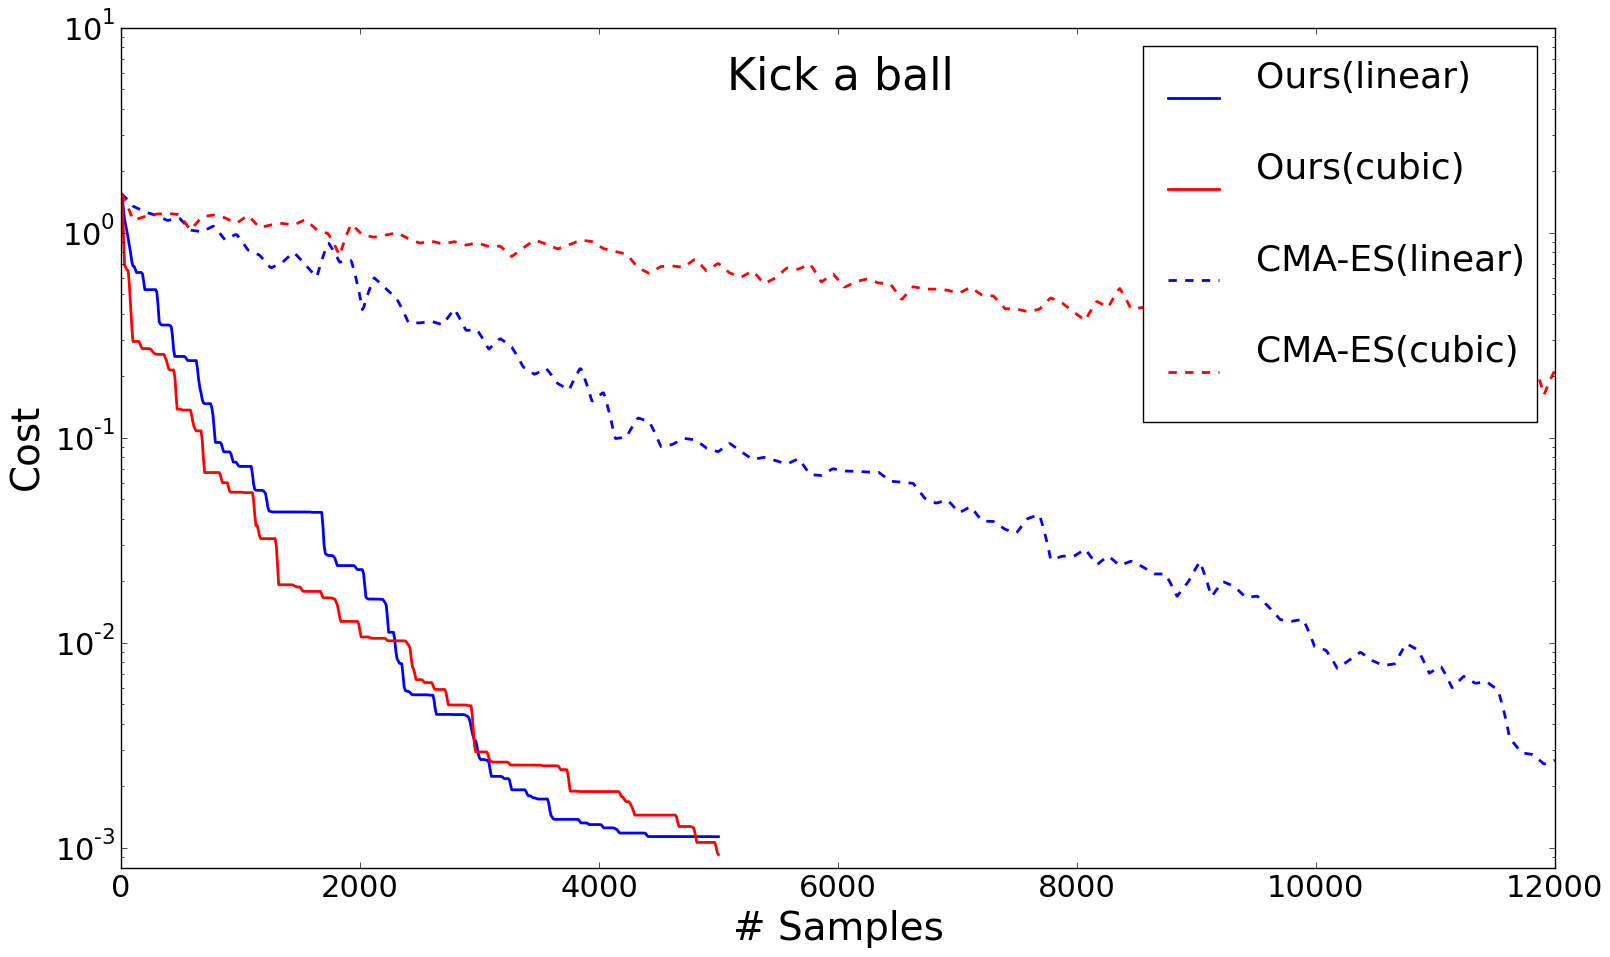
\includegraphics[width=4.5in]{images/iter_values_01}
  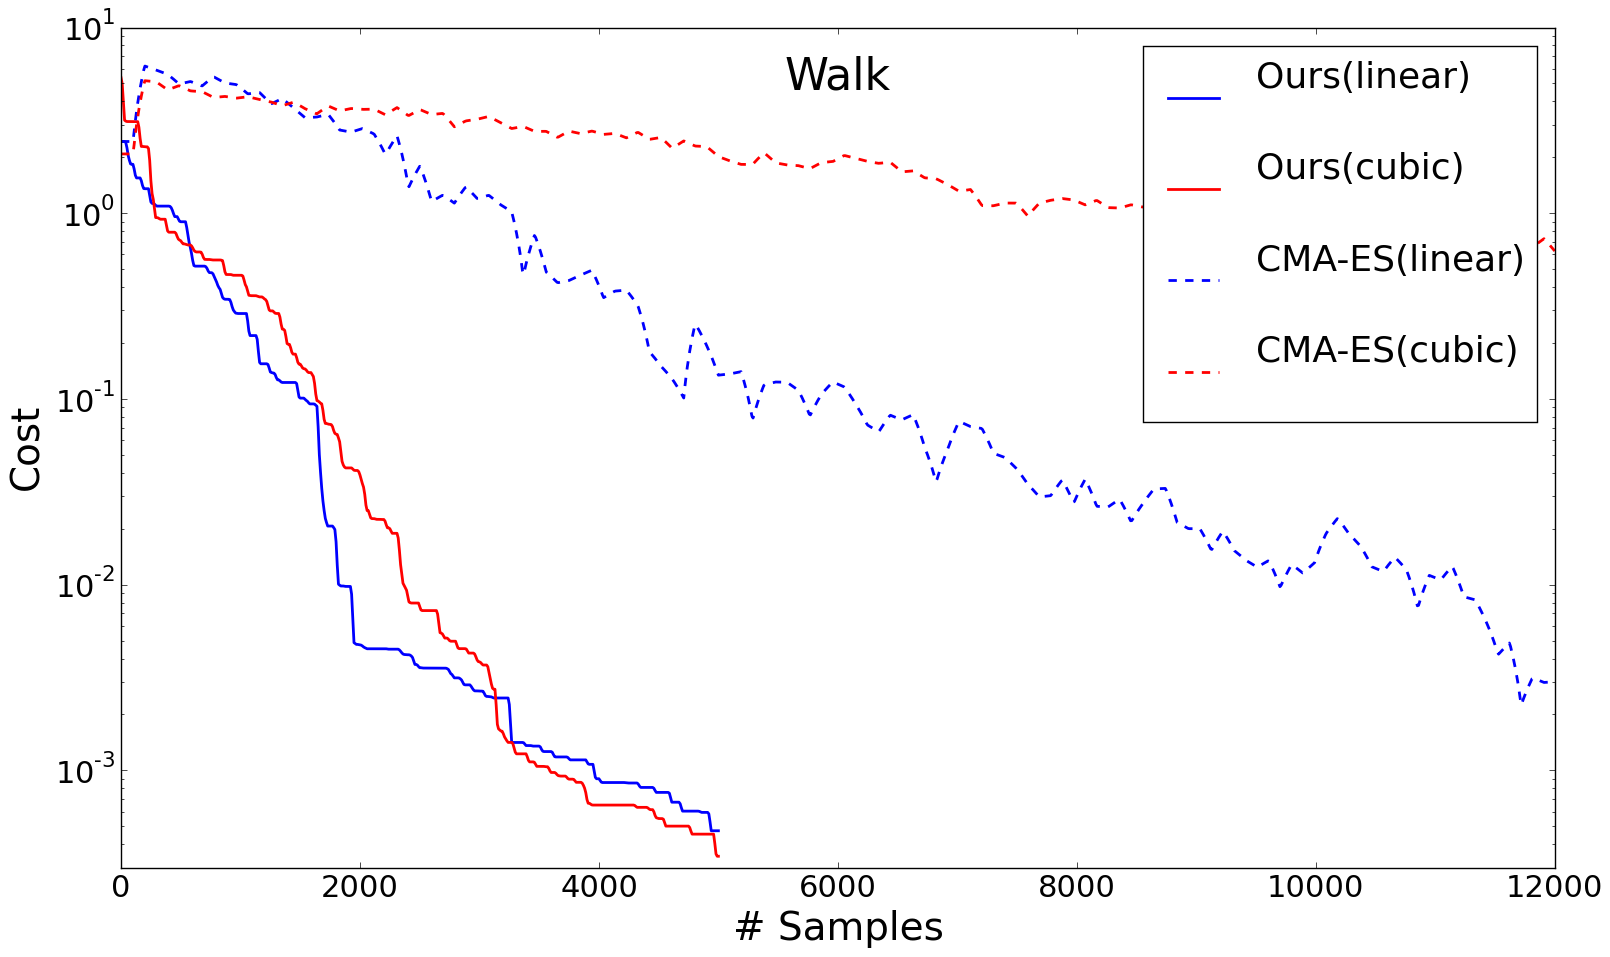
\includegraphics[width=4.5in]{images/iter_values_02}
  \caption{Comparison on three parameterized control problems. The
    cost (\eqnref{optskills_disccost}) is computed by averaging seven
    optimization trials. In all problems, our algorithm converges
    faster than CMA-ES, especially when the parameterized skill
    function is of cubic form.}
    % \updated{This plot shows the average cost (\eqnref{optskills_disccost}) over sample
    %   evaluations fort hree motion problems (Top: jumping, Middle:
    %   We present results of our algorithm (solid) and CMA-ES (dashed) with two
    %   mean segments, linear(red) and cubic(blue).
    %   In all problems, our algorithm converges faster than CMA-ES, especially
    %   when we use a cubic mean segment.  }
  
  \label{fig:optskills_iter_values}
\end{figure}

%% \begin{table}
%% \center
%% {
%% \caption{\updated{The comparison of our algorithm and CMA-ES on parameterzed
%%     motor skill problems.}}
%% \begin{tabular}{| c c | c c | c c |}
%% \hline
%% & & \multicolumn{2}{c|}{Avg. \# iters} &
%% \multicolumn{2}{c|}{Avg. final cost} \\ \hline
%% Task & Dim & Ours & CMA-ES & Ours & CMA-ES \\ \hline
%% Jump & 6 & 5000 & 5000 & 0.0055 & 0.0926 \\ \hline
%% Kick & 6 & 5000 & 5000 & 0.0228 & 0.1288 \\ \hline
%% Walk & 7 & 5000 & 5000 & 0.0400 & 0.5158 \\ \hline
%% \end{tabular}
%% \label{tab:optskills_motor_result}
%% }
%% \end{table}

\subsubsection{Vertical Jump}
Our goal is to learn a parameterized vertical jump skill ranging from
$3cm$ to $8cm$.
We designed two objective terms to achieve desired motion: the
balance term and the apex height of center of mass.
\begin{equation}
  f_{jump}(\vc{x}; w) =
  \|\vc{h}_{balance}(\mathcal{S}(\vc{x}))\|^2 + 
  ( h_{apex} (\mathcal{S}(\vc{x})) -  
  ((1-w)\hat{h}_{apex}^{0} + w\hat{h}_{apex}^{1}) )^2
\end{equation} 
  where $h_{apex}(\mathcal{S}(\vc{x}))$ evaluates the height of
  center of mass at apex of the jump. We set $\hat{h}_{apex}^{0} = 0.22$ and $\hat{h}_{apex}^{1} = 0.27$
  since the robot's center of mass height is $0.19m$ at the rest
  pose.
%%   $\vc{h}_{balance}(\mathcal{S}(\vc{x}))$ evaluates the balance
%%   of the motion using the following cost function:
%% \begin{equation}
%% \vc{h}_{balance}(\mathcal{S}(\vc{x})) = \sum_{\vc{s}_i\in\mathcal{S}(\vc{x})}\|\vc{C}_{xz}(\vc{s}_i)-\vc{P}_{xz}(\vc{s}_i)\|^2
%% \end{equation}
%% \updated{where $\vc{C}_{xz}(\vc{s}_i)$ and $\vc{P}_{xz}(\vc{s}_i)$ are the
%%   horizontal positions of the center of mass and the center of pressure for the
%%   given state $\vc{s}_i$.}
  %% \karen{Define notations and explain the equation.}
  $\vc{h}_{balance}(\mathcal{S}(\vc{x}))$ evaluates the state of
  balance by computing the squared sum of horizontal distances between
  the center of mass and the center of pressure over the entire
  motion.

%% The target center of mass $max\{\vc{C}\}$ is $[0,
%% 0.22, 0]^T$ at $w=0$ and $[0, 0.27, 0]^T$ at $w=1$ since a robot's
%% standing COM height is $0.19$. \karen{Why don't we just show Equation
%%   9 customized to this cost function?}
We broke a vertical jump into
three phases: preparing, thrusting, and landing.
The policy $\pi_{jump}$ is
then defined by six parameters: the target hip, knee, and ankle angles during
preparing phase, the intended magnitude of force exerted to the ground during
thrusting phase, and the target hip and knee angles during landing phase.

Because the humanoid hardware is not sufficiently powerful to perform
vertical jumps, we remove the torque limits during the
thrusting phase.

\subsubsection{Kick a Ball}
Inspired by the work on quadrupeds playing soccer
%% \karen{Is this correct description of the paper?}
\cite{Hausknecht:2010:LPK}, the goal of this example is to learn a parameterized skill to kick a ball such that it travels a desired distance ranging from
$0.3m$ to $0.6m$.
Although in previous work a quadruped was allowed to fall
after kicking a ball, we required our biped humanoid to maintain an
upright balanced posture throughout the entire motion.
The objective function is defined as follows:
\begin{equation}
  f_{kick}(\vc{x}; w) =
  \|\vc{h}_{balance}(\mathcal{S}(\vc{x}))\|^2 + 
  \| \vc{h}_{ball} (\mathcal{S}(\vc{x})) -  
  ((1-w)\hat{\vc{h}}_{ball}^{0} + w\hat{\vc{h}}_{ball}^{1}) \|^2
\end{equation} 
  where $\vc{h}_{ball}(\mathcal{S}(\vc{x}))$ is the final position of the ball, $\hat{\vc{h}}_{ball}^{0}$ is $[0, 0.03, 0.3]^T$, and
  $\hat{\vc{h}}_{ball}^{1}$ is $[0, 0.03, 0.6]^T$.
We broke the motion into three phases: leg
lifting, backward leg swing, and forward leg swing, with six
parameters for policy $\pi_{kick}$:
the target hip angle during leg lifting, the target hip and knee
angles during backward leg swing, and the target hip, knee, and ankle angles during forward leg swing.
%% \karen{which three angles?}

\subsubsection{Walk}
The goal is to learn a locomotion controller such that the humanoid
can walk at different speeds ranging from $6.7cm/s$ to
$13.3cm/s$. We measured the walking speed over three seconds of
simulation. The objective function is defined as
\begin{equation}
  f_{walk}(\vc{x}; w) =
  \|\vc{h}_{balance}(\mathcal{S}(\vc{x}))\|^2 + 
  \| \vc{h}_{com} (\mathcal{S}(\vc{x})) -  
  ((1-w)\hat{\vc{h}}_{com}^{0} + w\hat{\vc{h}}_{com}^{1}) \|^2
\end{equation} 
where $\vc{h}_{com}(\mathcal{S}(\vc{x}))$ is the center of mass
position at the final frame, $\hat{\vc{h}}_{com}^{0}$ is $[0, 0.19, 0.15]^T$, and
$\hat{\vc{h}}_{com}^{1}$ is $[0, 0.19, 0.40]^T$. One step of walk (half gait cycle)
consists of three phases: take-off (foot leaving the ground)
%% \karen{describe what each phase means in paramethesis}),
swing (leg swinging forward), and contact (the other foot touching
the ground).  We defined seven parameters for policy $\pi_{walk}$
including the duration of the swing phases, the target hip, knee,
and ankle angles for the take-off phase, and the target hip, knee,
and ankle angles for the swing phase. We started from a manually
designed policy which produces successful walk at $8.5cm/s$. Based
on the parameter values of this manual controller, we set the bounds for
the policy parameters in the optimization.


  % and add policy parameters that can adjust the target poses and timing.
  % One step of walking consists of three phases: \emph{lifting}, \emph{swinging},
  % and \emph{landing}.
  % After the step, the target poses of phases are mirrored for the next step.
  % The seven policy parameters are a duration of \emph{swinging} phases and three
  % lower body joint angles for both \emph{lifting} and \emph{swinging} phases.

\subsubsection{Results}
We compared our algorithm and CMA-ES with the linear parameterized skill
function, as well as the cubic one. Our algorithm outperforms CMA-ES in
all three problems (\figref{optskills_iter_values}). When solving linear
parameterized skill functions, CMA-ES required
approximately $2.5$ times more samples than our algorithm. When
solving cubic parameterized skill functions, our algorithm yielded a
better solution with almost no slowdown in convergence. CMA-ES, on the
other hand, became extremely slow and could not find any good solution
when terminated at maximal iterations ($12000$). Comparing the
difference in linear and cubic parameterized skill functions on our
algorithm, an interesting observation is that, among three motor
skills, cubic parameterization results in significant improvement only
for the vertical jump problem. We conjecture the reason being that the intended force exerted to the
ground during the thrusting phase has a highly nonlinear relationship with the resulting height
of the jump. A cubic parameterized skill function captures this
nonlinearity better than the linear one.

%   We allow $5000$ sample evaluations for our
% algorithm and $12000$ for CMA-ES.  In general, our algorithm shows the
% faster convergence than CMA-ES for all three motions
% (\figref{optskills_iter_values}).  For the linear mean segment, CMA-ES requires
% approximately $2.5$ times more samples than our algorithm.  When we
% extend a form of the mean segment to cubic, our algorithm shows almost
% similar convergence rate and finds a lower final cost, while CMA-ES
% becomes drastically slower.  Although a cubic mean function clearly
% outperforms only for jumping that requires non-linear magnitude of
% forces at \emph{thrusting} stage, but we expect that it will can be
% applied to a wider range of dynamic motions.

\begin{figure}
\center
  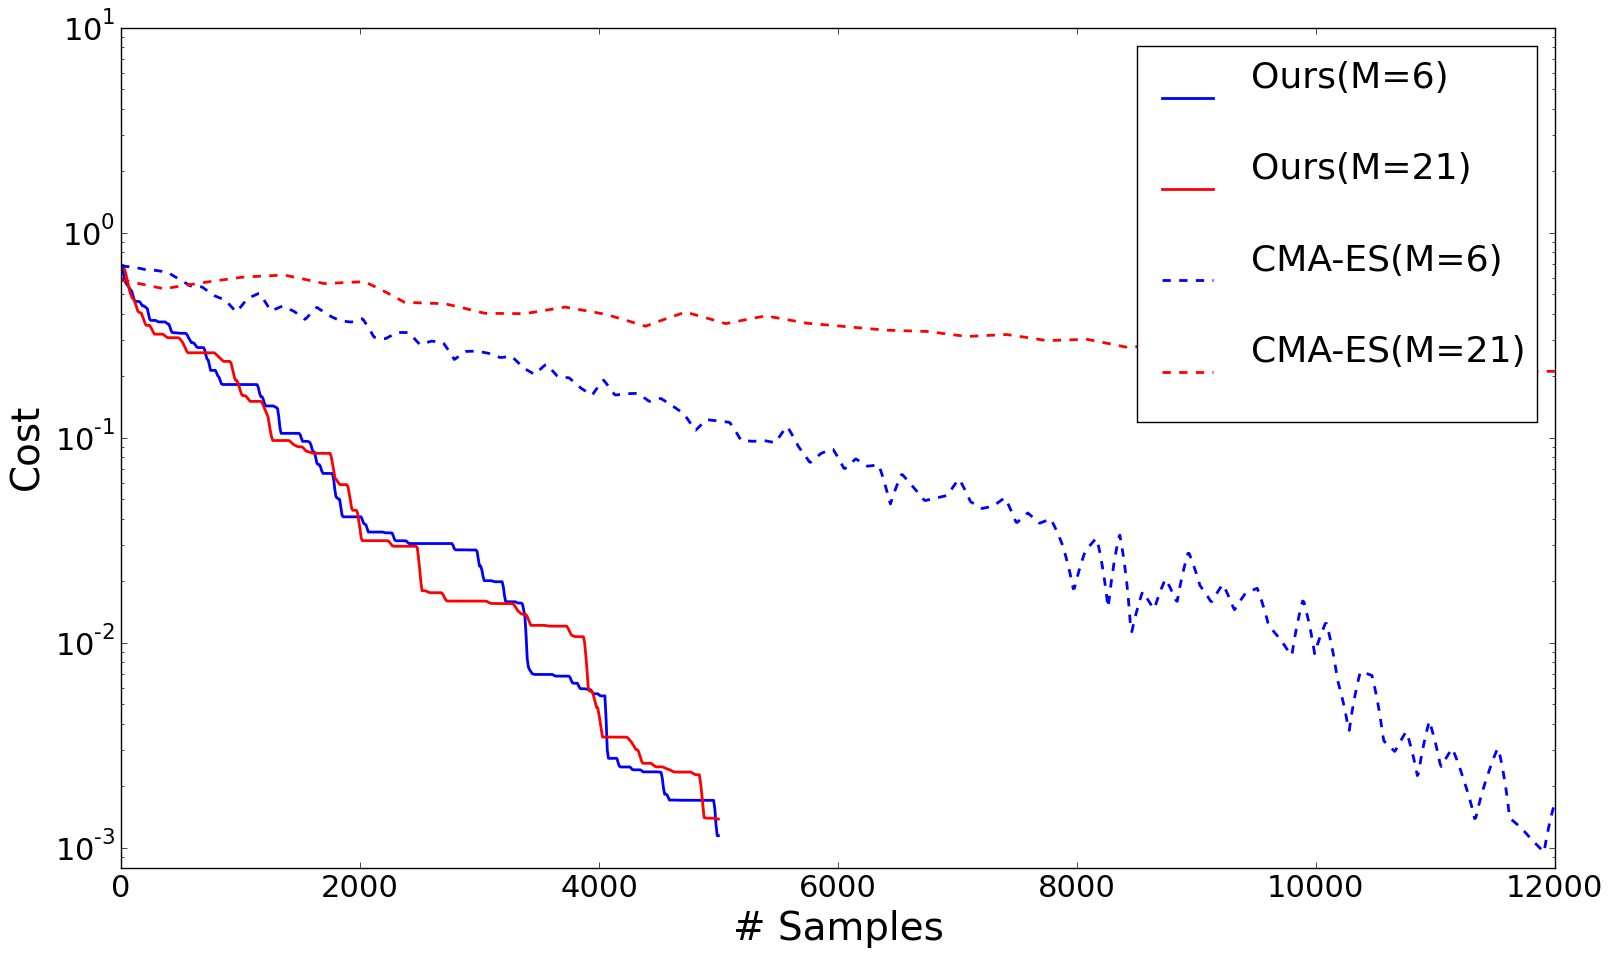
\includegraphics[width=4.0in]{images/diff_M}
  \caption{The impact of task discretization on convergence. More
    discrete tasks slow down the convergence of CMA-ES significantly,
    while it has negligible impact on our algorithm.}

  %   \updated{The plot shows the changes of convergence of our algorithm (solid)
  %     and CMA-ES (dash) on the jumping task when we increase the number of
  %     discrete task interpolation parameters $M$ from $6$ (blue) to $21$ (red). 
  %     The more task parameters slows down the convergence of CMA-ES by three to
  %     four times, while has less significant impact on our algorithm. }
  % }
  \label{fig:optskills_diff_m}
\end{figure}

In addition, we investigated the impact of task discretization on the
convergence rate. Specifically, we solved the
vertical jump problem using different numbers of discrete tasks, $M =
6$ and $M = 21$, and compared the results in \figref{optskills_diff_m}. Although
finer discretization ($M=21$) should result in a better solution, it
slows down the convergence because more samples
evaluations are required. Since CMA-ES directly optimizes
$\hat{f}({\boldsymbol{\phi}})$, it becomes three to four times slower
when $M = 21$. On the other hand, \figref{optskills_diff_m} shows that our algorithm does not suffer from
  slower convergence rate when the number of discrete tasks increases.

% In addition, we compared the change of convergence rate on the jumping
%   task when the number of discrete tasks $M$ is increased from $6$ to $21$ 
%   (\figref{optskills_diff_m}). 
%   Although  more $M$ ensures the quality of motions for more tasks, it 
%   decelerates optimization by requiring more samples to evaluate 
%   the objective function $\hat{f}({\boldsymbol{\phi}})$.
%   %% We tested our algorithm and CMA-ES with two differnt $M$ values, $6$ and
%   %% $21$, on the jumping task (\figref{optskills_diff_m}).
%   %% We compared the effect of $M$ on convergence rate of our algorithm and
%   %% CMA-ES by testing two $M$ values ($6$ and $21$) on the jumping
%   %% task (\figref{optskills_diff_m}). 
%   Since CMA-ES directly optimizes $\hat{f}({\boldsymbol{\phi}})$, it becomes
%   three to four times slower.
%   On the other hand, deceleration is less obvious for our algorithm, which
%   is due to the existance of the elite pool that contains all the best
%   samples in the history.

%% \updated{We run our algorithm with $\mu=48(\nu=\mu/M=8), \lambda=16$.
%%   For comparison, CMA-ES runs with $\mu=8$ and $\lambda=16$.
%%   For the motion problems, we compared the average of the final
%%   values \tabref{optskills_motor_result}.
%%   %% We use geometric average to well illustrate the distribution.
%%   In general, our algorithm finds the better solution, ...
%%   Ocassionally, our algorithm also falls into the local minima (approximately
%%   10\% for our problems) when the initial guess was very bad.
%%   The qualitatively, CMA-ES produces very poor quality of motion that often
%%   falling, which means it is local minima.
%%   The quality of motion from our solution is quite good (\figref{optskills_motions}). }


%%%%%%%%%%%%%%%%%%%%%%%%%%%%%%%%%%%%%%%%%%%%%%%%%%%%%%%%%%%%%%%%%%%%%%%%%%%%%%%%

\subsection{Parameterized CEC'15 Problems}
\begin{table}
\center
{
\caption{Results on Parameterized CEC'15 Problems}
\begin{tabular}{| c c | c c | c|}
\hline
Function & Dim & Ours(evals) & CMA-ES(evals) & Ratio \\ \hline
Sphere & 5 & 6309.7 & 7151.1 & 0.88 \\ \hline
Sphere & 10 & 9460.3 & 13404.9 & 0.71 \\ \hline
Sphere & 20 & 16395.4 & 23539.7 & 0.70 \\ \hline
Bent-Cigar & 5 & 1402.6 & 2666.6 & 0.53 \\ \hline
Bent-Cigar & 10 & 3092.0 & 5724.9 & 0.54 \\ \hline
Bent-Cigar & 20 & 5824.3 & 11196.9 & 0.52 \\ \hline
\hline
Function & Dim & Ours(cost) & CMA-ES(cost) & Ratio \\ \hline
Weierstrass & 5 & 0.00093 & 0.03549 & 0.026 \\ \hline
Weierstrass & 10 & 0.00105 & 0.15398 & 0.007 \\ \hline
Schefel & 5 & 0.00444 & 0.07025 & 0.063 \\ \hline
Schefel & 7 & 0.00848 & 0.25131 & 0.034 \\ \hline
\end{tabular}
\label{tab:optskills_cec15_result}
}
\end{table}

We tested the performances of our algorithm and the baseline algorithm on four
parameterized problems from the benchmark CEC'15 \cite{Chen:2015:CEC} which was
designed for testing evolutionary optimization algorithms.  
We selected two unimodal problems (Sphere and Bent-Cigar) and two multimodal
problems (Weierstrass and Schwefel) from the benchmark set. 
However, the objective functions in CEC'15 were designed for testing
standard single-task optimizations rather than for parameterized
optimization problems. Therefore, we took the original objective function $f(\vc{x})$
and parameterized it by shifting, rotating, and scaling it with the
parameter $w$:
\begin{equation}
  \begin{aligned}
    f(\vc{x}; w) = s_w f(\mat{R}_w(\vc{x}-\vc{t}_w))
  \end{aligned}
\end{equation} 
where $\vc{t}_w, \mat{R}_w, s_w$ are linear functions of $w$ and
represent the shift, rotation, and scale parameters for the task
$w$. The parameterized skill function is assumed linear in $w$ for all four problems. 

The results are shown in \tabref{optskills_cec15_result}.  For unimodal
functions, we compared the average number of samples required to reach
the convergence threshold ($=0.001$). Our algorithm requires $52\% -88\%$ samples comparing
  to CMA-ES on Sphere and Bent-Cigar problems.
%% Since the convergence is not ensured for multimodal problems, we compared the
%% average final cost instead of the number of samples \karen{I don't see
%%   the causal relationship here.}.
For multimodal problems, comparing the number of samples is not
informative because one algorithm might use fewer samples but returns a
very bad local minimum, while the other spends more samples to find a
better local minimum or even the global one. Therefore, we compared
the cost of the solution found by each algorithm instead of the number
of samples used. For Weierstrass and Schwefel, the cost of solution
for our algorithm is $0.7\%-6.3\%$ of that of CMA-ES.
%% For Weierstrass and Schwefel, our algorithm finds the $0.7$\% to $0.0$ times lower
%% final cost while CMA-ES finds local minima
%% \karen{Again, compute the reciprocal.}.
From the four problems we evaluated, the performance gain increases as
the dimension of the problem grows, although further investigation with
more problem sets is needed to verify this trend.

%%%%%%%%%%%%%%%%%%%%%%%%%%%%%%%%%%%%%%%%%%%%%%%%%%%%%%%%%%%%%%%%%%%%%%%%%%%%%%%%
\subsection{Comparison with Individual Learning Approach}
\begin{figure}[h]
\center
  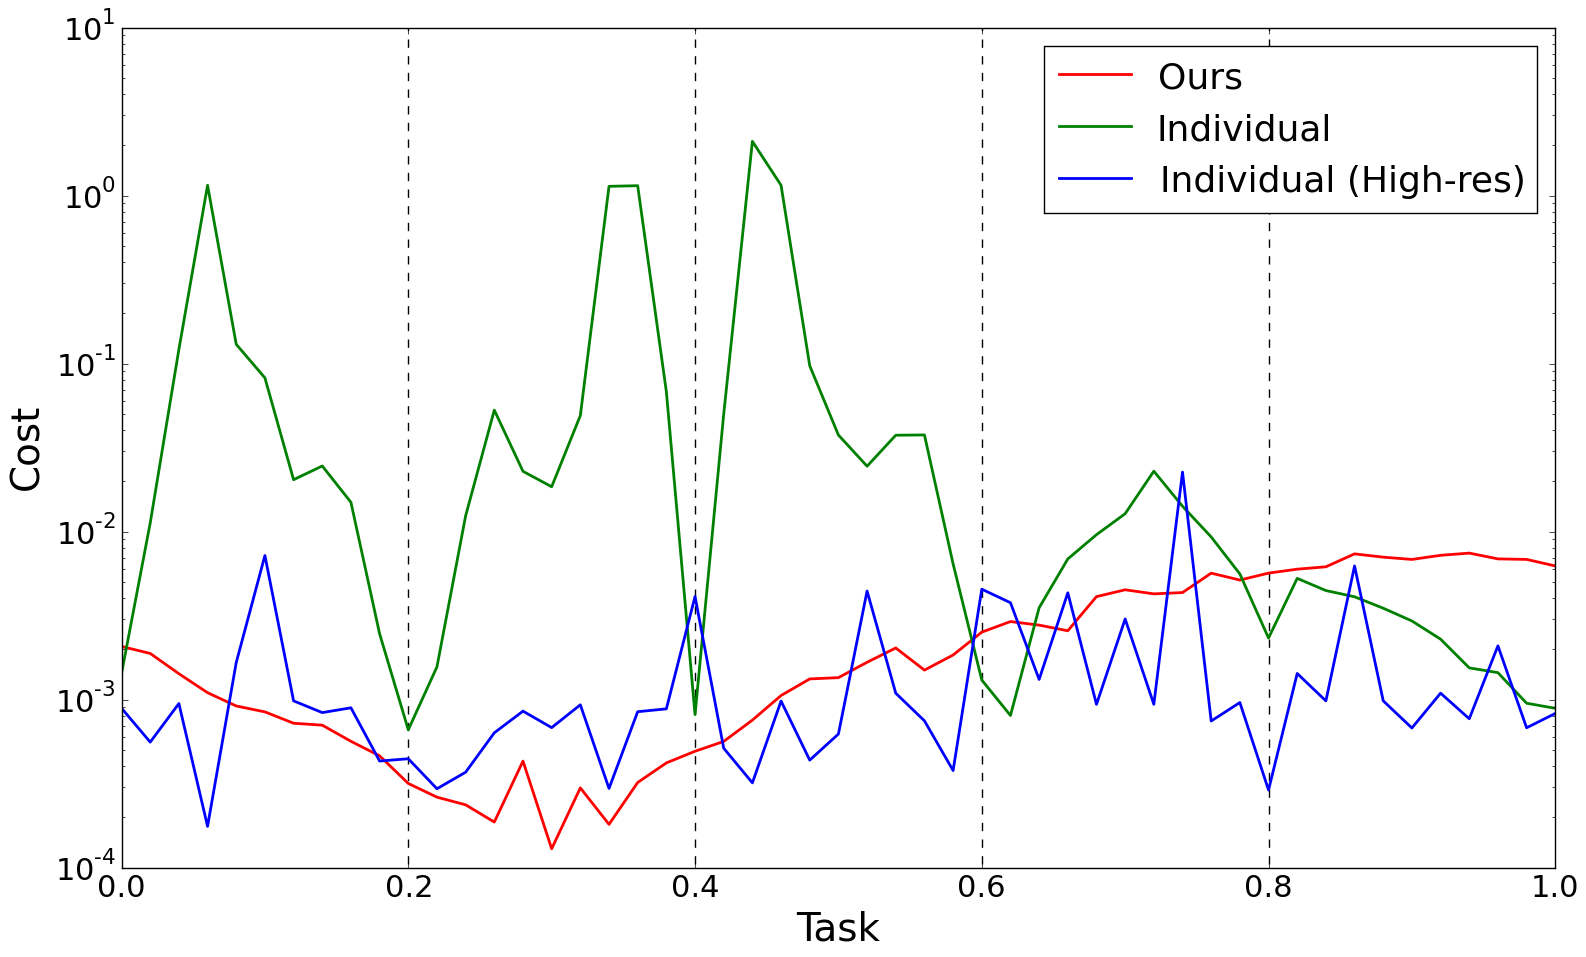
\includegraphics[width=4.5in]{images/plot_vs_ind}
  \caption{Comparison between our algorithm and the individual
    learning approach. The quality of the low-resolution policy
    (shown in green) is comparable with the high-resolution one (shown
    in blue) for those six tasks used for training (dotted vertical
    lines). However, for those tasks corresponding to interpolated
    policy parameters, there is a significant discrepancy between the
    quality of low-resolution and high-resolution policies. In
    contrast, our policy (shown in red) learned with only six tasks (M
    = 6) is comparable to the high-resolution one.}


  %   \updated{The plot shows the quality of control parameters for the
  %     interpolated tasks. 
  %     Our algorithm (red) and the individual learning approach (green) are
  %     trained for six tasks ($\vc{w} = \{0.0, 0.2, .. , 1.0\}$) and tested for
  %     $51$ tasks ($\vc{w}_{high} = \{0.0, 0.02, .., 1.0\}$).
  %     The quality is also compared to the ground truth, the individual learning
  %     with all $51$ tasks (blue).
  %     The solution of our algorithm shows the better performance than the
  %     individual learning approach for the unseen tasks, especially between
  %     $0.0$ and $0.6$.} 
  % }
  \label{fig:optskills_vs_ind}
\end{figure}

% \sehoon{Interpolate the neighbor parameters: ex)
%   $\vc{x}_{0.1}=0.5\vc{x}_{0.0}+0.5\vc{x}_{0.2}$. I tested on jumping
%   problem.}
Alternatively, a parameterized policy can be trained by defining a set
of tasks, learning a policy for each task separately, and
interpolating the policies using a regression model. We refer this
method as \emph{individual learning approach}. We solved the vertical
jump problem using individual learning approach with two different
resolutions of task discretization. In the low-resolution setting, we
individually learned six tasks evenly across the entire task range
(\ie $M = 6$) and applied linear regression on the learned policy
parameters. We repeated the same process in the high-resolution
setting except that this time we individually learned $51$ tasks (\ie
$M = 51$). The quality of the low-resolution policy is comparable
with the high-resolution one for those six tasks used for training
(dotted vertical lines in \figref{optskills_vs_ind}). However, for those tasks
corresponding to interpolated policy parameters, there is a significant
discrepancy between the quality of low-resolution and
high-resolution policies. In contrast, our policy learned with only
six tasks ($M=6$) is comparable to the high-resolution
one.

% To compare our algorithm and individual
% approach for unseen situations, we train controllers with sparse tasks
% ($M=6$) and test on high resolution tasks $\vc{w}_{high} = \{0.0,
% 0.02, .., 1.0\}$ where $M_{high}=51$.  In \figref{optskills_vs_ind}, both
% controllers show good performances for six trained tasks (dotted
% vertical lines).  However, our model produces the better solutions for
% new tasks, especially between $0.0$ and $0.6$.  In fact, the quality
% of our solution is comparable to a solution of individual approach
% with high resolution tasks, which is considered as ground truth.

%%%%%%%%%%%%%%%%%%%%%%%%%%%%%%%%%%%%%%%%%%%%%%%%%%%%%%%%%%%%%%%%%%%%%%%%%%%%%%%%
\subsection{Hardware experiment}
\begin{figure}
\center
  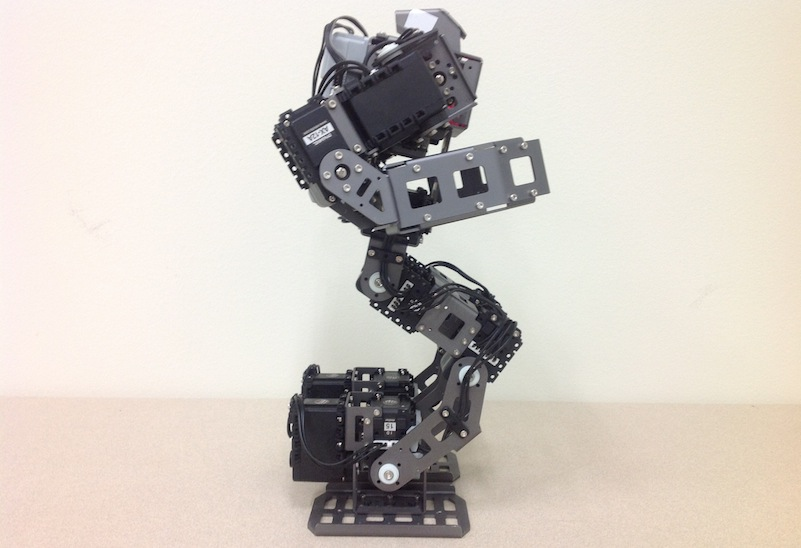
\includegraphics[width=3.0in]{images/hardware}
  \caption{
    BioloidGP hardware.
  }
  \label{fig:optskills_hardware}
\end{figure}
Our evaluation also includes deploying the learned walking policy on
the hardware (\figref{optskills_hardware}). The only difference in the
parameterized policy for the real robot is that we decreased the
bounds of the policy parameters during the optimization. This
reduction results in more stable walk but decreases the maximal target
speed from $13.3cm/s$ to $10.0 cm/s$.

% Although we used the initial controller that is
% successful on hardware, there is no guarantee that the parameterized
% controller will be also successful.  To increase the success rate, we
% set the smaller domain for parameters so that the controller behaves
% similarly to the initial controller and decrease the maximum target
% speed from 13.3cm/s to 10.0 cm/s.  As a result, the new controller can
% successfully walk with different speeds on the hardware (please refer
% the video).
  %% The smaller domain leads to change of the strategy: the robot took larger
  %% steps for fast walking, but now it takes faster steps.}
